
% --------------------------------------------------------------- CONFIGURATIONS

%ifdef TWOSIDE
	%\documentclass[a4paper,12pt,final,twoside,openright]{book}
%elif ONESIDE
	\documentclass[a4paper,12pt,final,oneside]{book}
%endif

\usepackage{report}
\usepackage{mathtools}
\usepackage[font=small, labelfont=bf]{caption}


% -------------------------------------------------------------- META: CONSTANTS

\newcommand{\reporttitle}{Digital Image Processing}
\newcommand{\reportauthor}{Thierry~\textsc{Cantenot}}
\newcommand{\reportsubject}{Report}
\newcommand{\topic}{Assignments}
\newcommand{\HRule}{\rule{\linewidth}{0.5mm}}
\setlength{\parskip}{1ex} % Espace entre les paragraphes

\hypersetup{
	pdftitle={\reporttitle},%
    pdfauthor={\reportauthor},%
    pdfsubject={\reportsubject},%
}

\title{\reporttitle}
\author{\reportauthor}
%\setcounter{tocdepth}{4}


% ------------------------------------------------------------------------- FILE

\begin{document}


    % ------------------------------------------------------------------- HEADER

	\renewcommand{\chaptername}{} %\renewcommand{\thechapter}{}
	\renewcommand{\contentsname}{Summary}

	\pagestyle{empty}
	\pagenumbering{Roman}


    % ------------------------------------------------------------ HEADER: TITLE

	\begin{flushleft}
    \textbf \reportauthor
\end{flushleft}

\vspace{2.0cm}

\begin{center}
	\textsc{\Large \reportsubject}\\[0.3cm]
	\HRule \\[0.4cm]
	{\Huge \bfseries \reporttitle}\\[0.3cm]
	{\LARGE \bfseries «~\topic~»}\\[0.3cm]
	\HRule \\[1cm]

	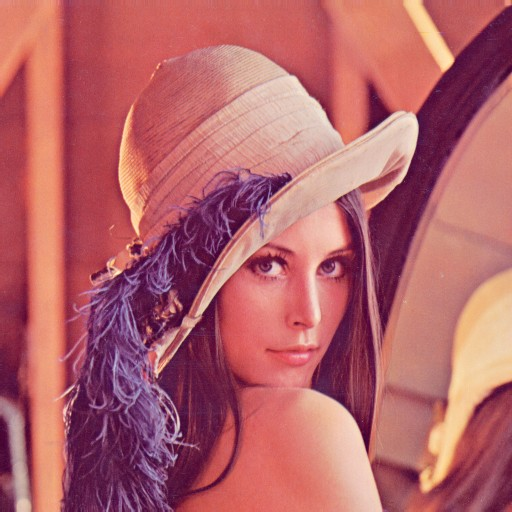
\includegraphics [scale=0.6]{images/lenna.jpg} \\[0.7cm]

	\vfill

    \begin{flushright}
        
\includegraphics[width=40mm]{images/SJTU_Logo.png}
    \end{flushright}

	\footnotesize{2014-2015}
\end{center}


	%ifdef TWOSIDE
		%\cleardoublepage
	%endif

	%\include{title2}

	%ifdef TWOSIDE
		%  \newpage
		%	\null
		%	\vfill
	%endif


    % --------------------------------------------------- HEADER: CONFIGURATIONS

	\sloppy          % Justification moins stricte : des mots ne dépasseront pas des paragraphes

    \frontmatter
		\pagestyle{empty}
		\tableofcontents
		\addtocontents{toc}{\protect\thispagestyle{empty}}

	\mainmatter
	\pagestyle{headings}

	\renewcommand{\thechapter}{\Alph{chapter}}
	\renewcommand{\chaptermark}[1]{\markboth{\MakeUppercase{\chaptername\ \thechapter.\ #1}}{}}
	\renewcommand{\sectionmark}[1]{\markright{\thesection{} #1}}


    % ------------------------------------------------------------------ CONTENT

    %\chapter{Histogram Equalization}

\section{Problem statement}

\begin{enumerate}
    \item Write a computer program for computing the histogram of an image.\\
    \item Implement the histogram equalization technique.\\
    \item Your program must be general to allow any gray-level image as its input.\\
\end{enumerate}

\section{Python implementation}

Usage:~\textbf{python problem1.py [-h] image\_path}
Use \textbf{python problem1.py -h} to see the help.

\pagebreak
\section{Figure 1}

    \subsection{Histogram}

    Original image:~\ref{diagram:fig1} |
    Original image's histogram:~\ref{diagram:hist_fig1}

    \begin{figure}[!htb]\centering
        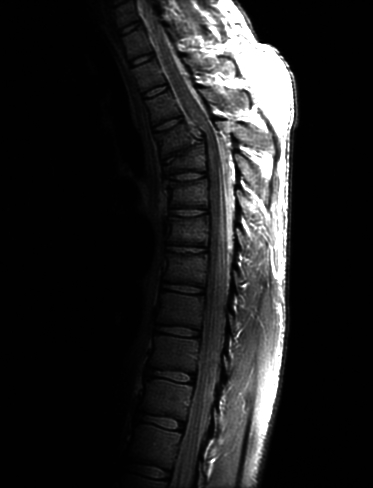
\includegraphics[width=0.5\linewidth]{./images/1/Fig1.jpg}
        \caption{Original \textit{Fig1.jpg}}\label{diagram:fig1}
    \end{figure}

    \begin{figure}[!htb]\centering
        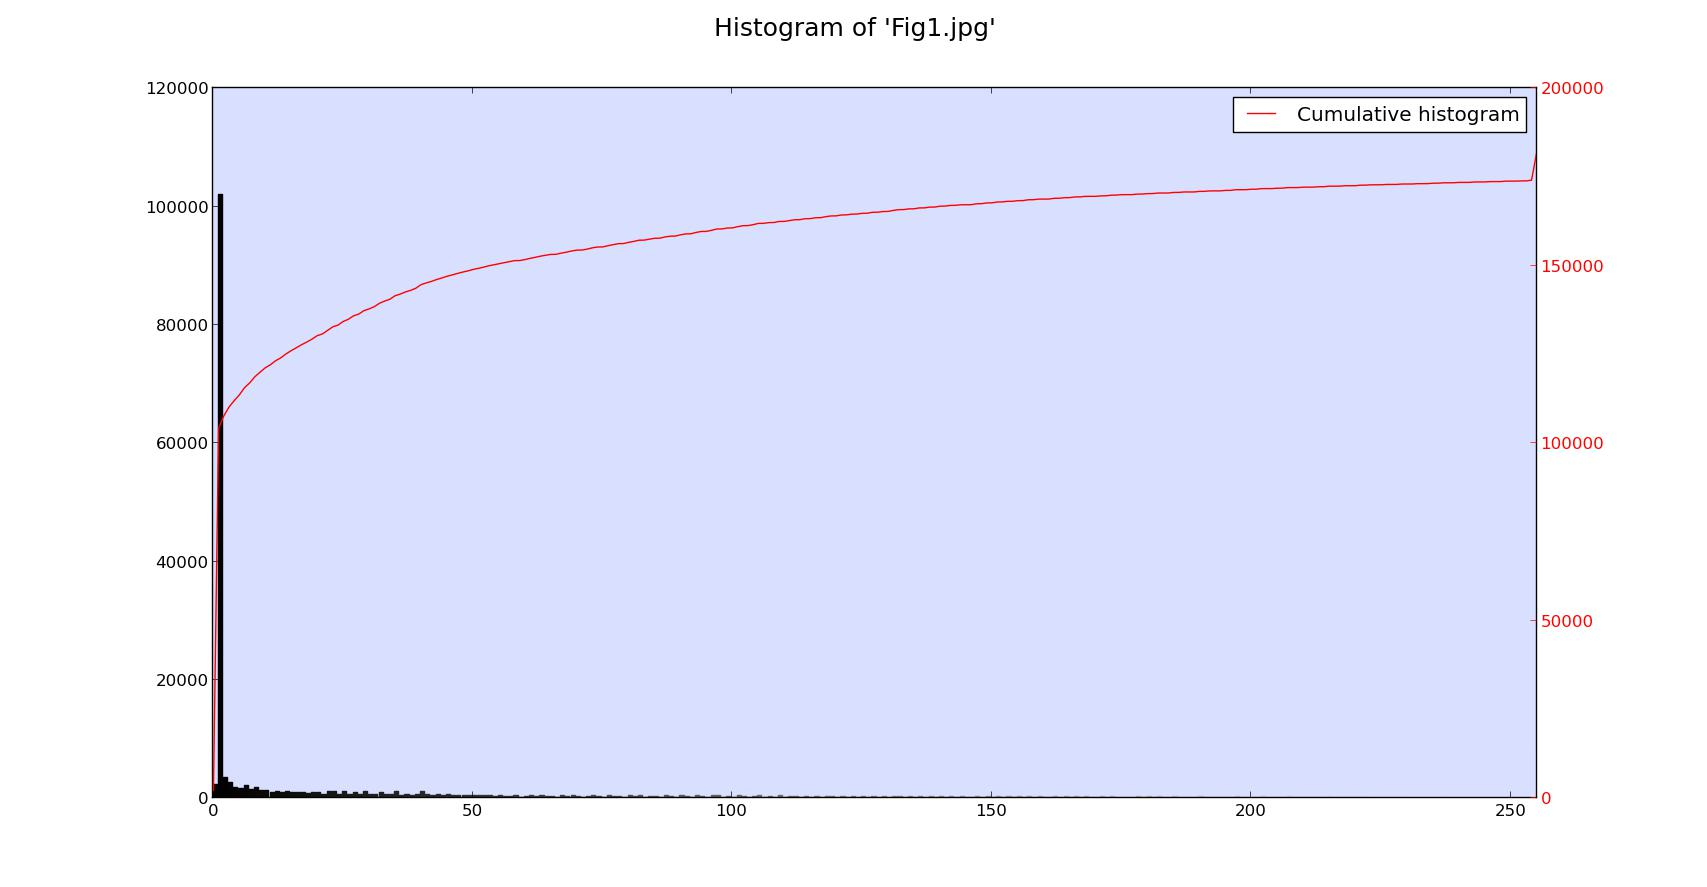
\includegraphics[width=\linewidth]{./images/1/Histogram_Fig1.jpg}
        \caption{Histogram of \textit{Fig1.jpg}}\label{diagram:hist_fig1}
    \end{figure}

    \pagebreak
    \subsection{Histogram equalization}

    Enhanced image:~\ref{diagram:enhanced_fig1} |
    Enhanced image's histogram:~\ref{diagram:equal_hist_fig1}

    \begin{figure}[!htb]\centering
        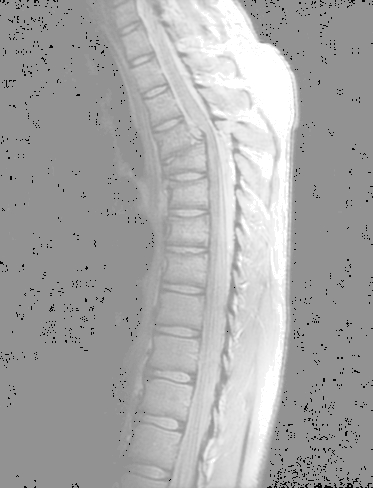
\includegraphics[width=0.5\linewidth]{./images/1/Enhanced_Fig1.jpg}
        \caption{Enhanced \textit{Fig1.jpg}}\label{diagram:enhanced_fig1}
    \end{figure}

    \begin{figure}[!htb]\centering
        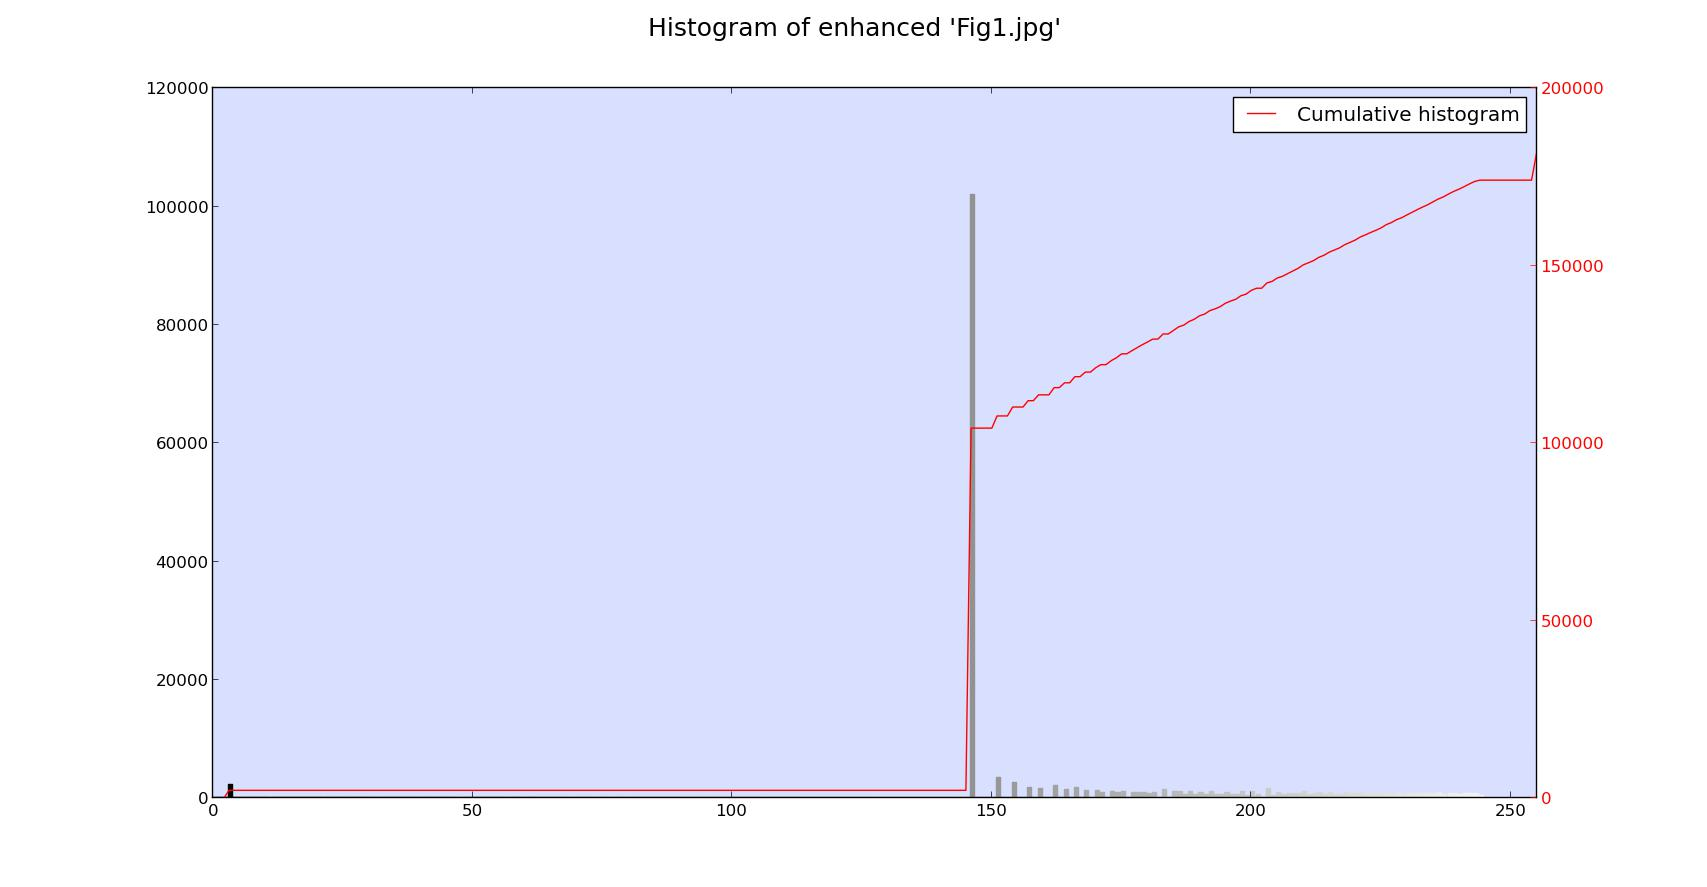
\includegraphics[width=\linewidth]{./images/1/Equalized_Histogram_Fig1.jpg}
        \caption{Equalized histogram of \textit{Fig1.jpg}}\label{diagram:equal_hist_fig1}
    \end{figure}


\pagebreak
\section{Figure 2}

    \subsection{Histogram}

    Original image:~\ref{diagram:fig2} |
    Original image's histogram:~\ref{diagram:hist_fig2}

    \begin{figure}[!htb]\centering
        
\includegraphics[width=0.5\linewidth]{./images/1/Fig2.jpg}
        \caption{Original \textit{Fig2.jpg}}\label{diagram:fig2}
    \end{figure}

    \begin{figure}[!htb]\centering
        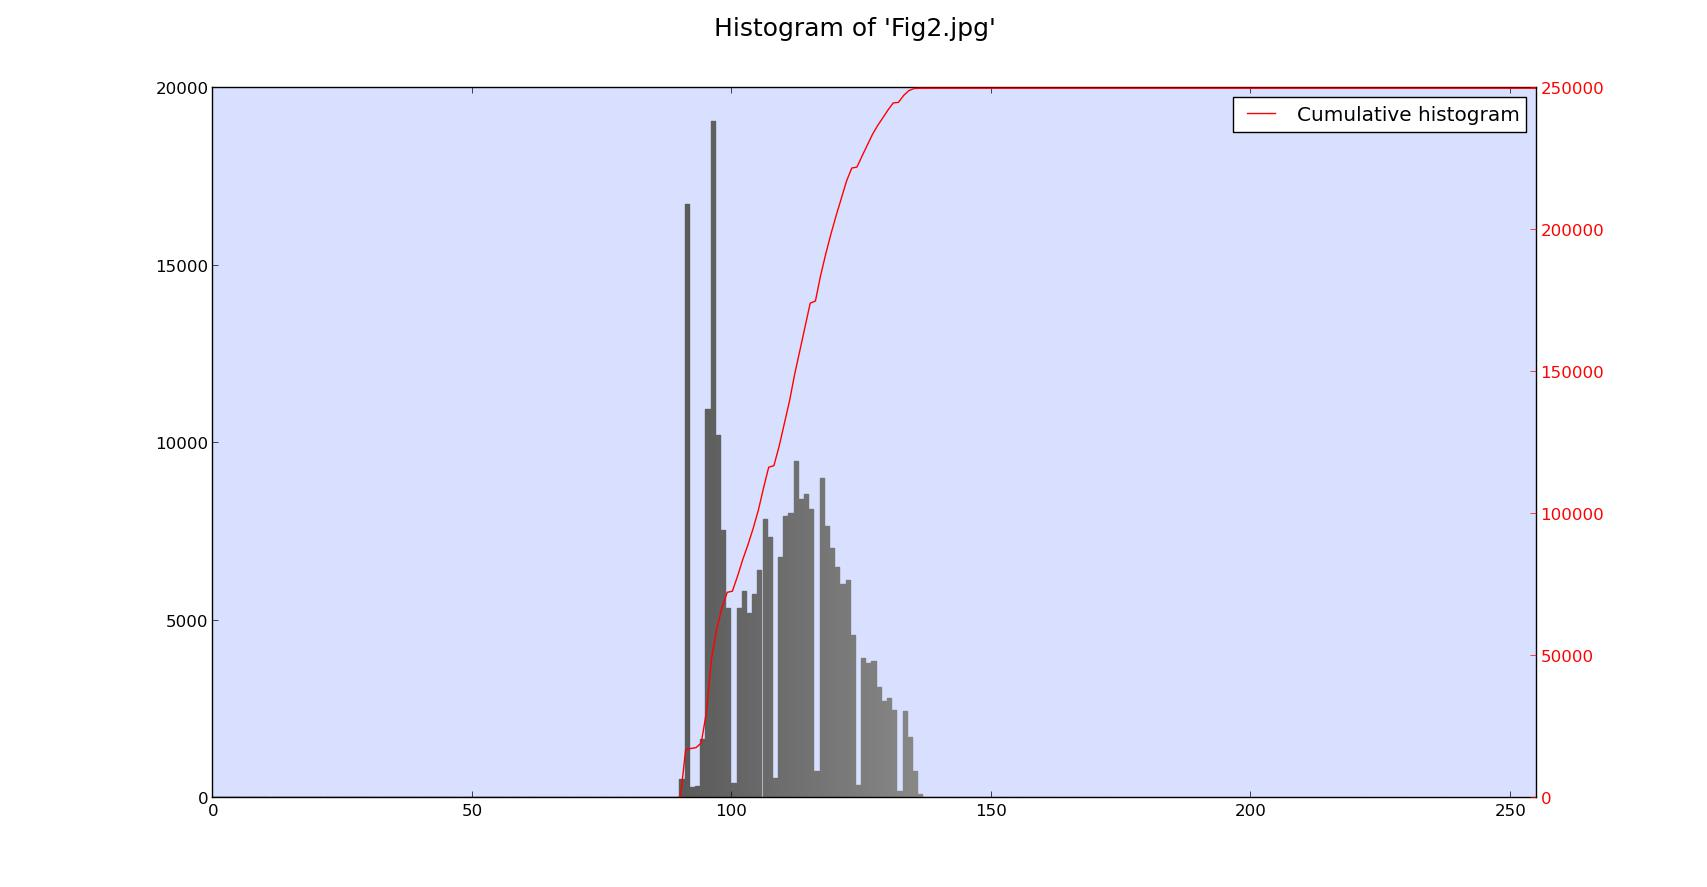
\includegraphics[width=\linewidth]{./images/1/Histogram_Fig2.jpg}
        \caption{Histogram of \textit{Fig2.jpg}}\label{diagram:hist_fig2}
    \end{figure}

    \pagebreak
    \subsection{Histogram equalization}

    Enhanced image:~\ref{diagram:enhanced_fig2} |
    Enhanced image's histogram:~\ref{diagram:equal_hist_fig2}

    \begin{figure}[!htb]\centering
        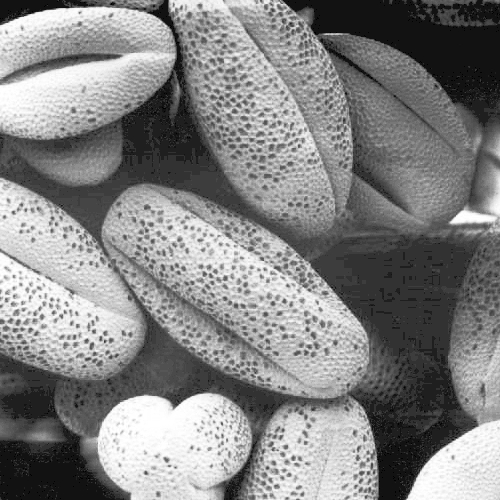
\includegraphics[width=0.5\linewidth]{./images/1/Enhanced_Fig2.jpg}
        \caption{Enhanced \textit{Fig2.jpg}}\label{diagram:enhanced_fig2}
    \end{figure}

    \begin{figure}[!htb]\centering
        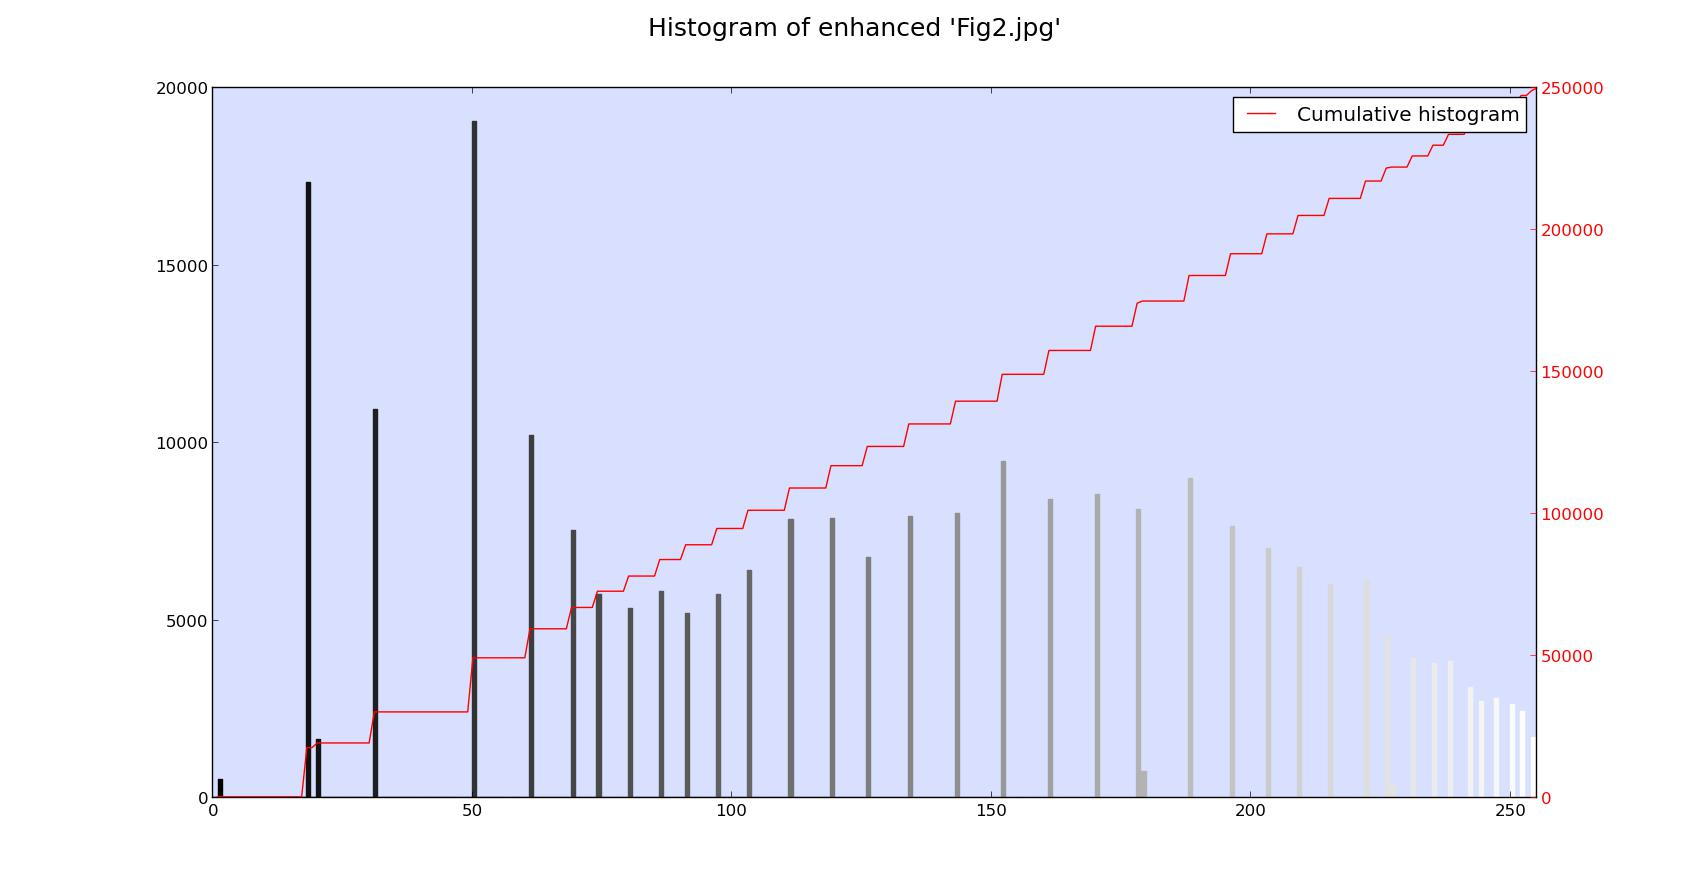
\includegraphics[width=\linewidth]{./images/1/Equalized_Histogram_Fig2.jpg}
        \caption{Equalized histogram of \textit{Fig2.jpg}}\label{diagram:equal_hist_fig2}
    \end{figure}

    %\chapter{Spatial enhancement methods}

\section{Problem statement}

Implement the image enhancement task of Section 3.7 (Fig 3.43) (Section 3.8, Fig 3.46 in our slides).\\
The image to be enhanced is \textit{skeleton\_orig.tif}.\\
You should implement all steps in Figure 3.43. \\

\section{Python implementation}

Usage:~\textbf{python problem2.py [-h] [--laplacian] [--sobel] [-a A] image\_path} \\

For example, to use a 3x3 Laplacian filter with A = 1.7, and then a Sobel, type:~\\
\textbf{python problem2.py --laplacian -a 1.7 --sobel skeleton\_orig.tif}

%The original image, its Laplacian, its sharpened (Laplacian) and its Sobel will be displayed.

\section{Results}

    \subsection{Original image}

    Original image:~\ref{diagram:skeleton}

    \begin{figure}[!htb]\centering
        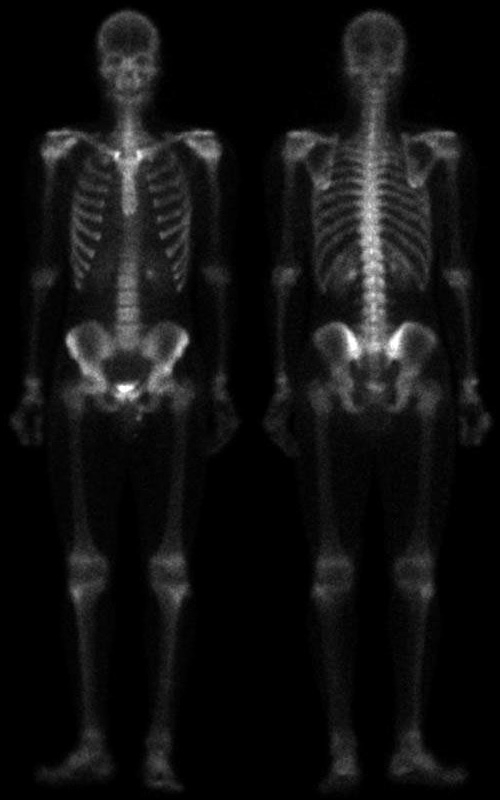
\includegraphics[width=0.7\linewidth]{./images/2/skeleton.jpg}
        \caption{Original \textit{skeleton\_orig.tif}}
        \label{diagram:skeleton}
    \end{figure}


    \subsection{3x3 Laplacian (A = 0)}

    Original image's laplacian:~\ref{diagram:laplacian_0} |
    Original image's sharpened laplacian:~\ref{diagram:laplacian_0_sharpened}

    \begin{figure}[!htb]\centering
        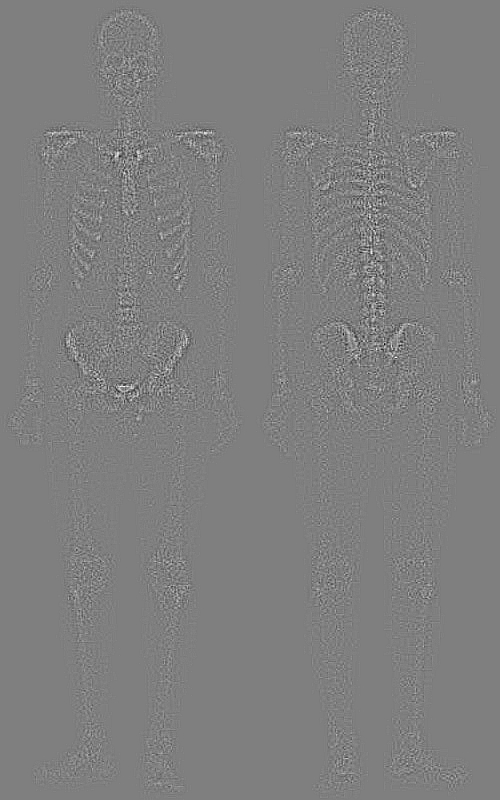
\includegraphics[width=0.4\linewidth]{./images/2/laplacian_A0.jpg}
        \caption{Laplacian (A=0)}\label{diagram:laplacian_0}
    \end{figure}

    \begin{figure}[!htb]\centering
        \begin{minipage}{0.40\textwidth}
            \frame{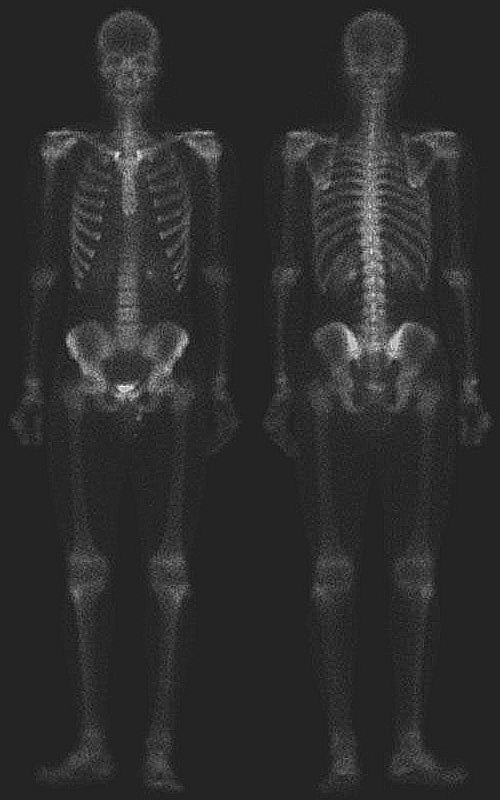
\includegraphics[width=\linewidth]{./images/2/laplacian_A0_sharpened.jpg}}
            \caption{Sharpened image}\label{diagram:laplacian_0_sharpened}
        \end{minipage}
        \begin{minipage}{0.40\textwidth}
        \frame{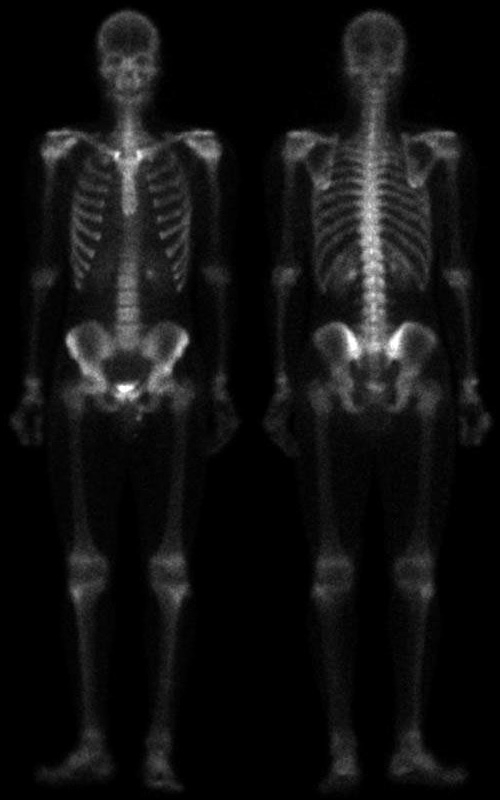
\includegraphics[width=\linewidth]{./images/2/skeleton.jpg}}
        \caption{Original image}
        \end{minipage}
    \end{figure}


    \subsection{3x3 Laplacian (A = 1)}

    Original image's laplacian:~\ref{diagram:laplacian_1} |
    Original image's sharpened laplacian:~\ref{diagram:laplacian_1_sharpened}

    \begin{figure}[!htb]\centering
        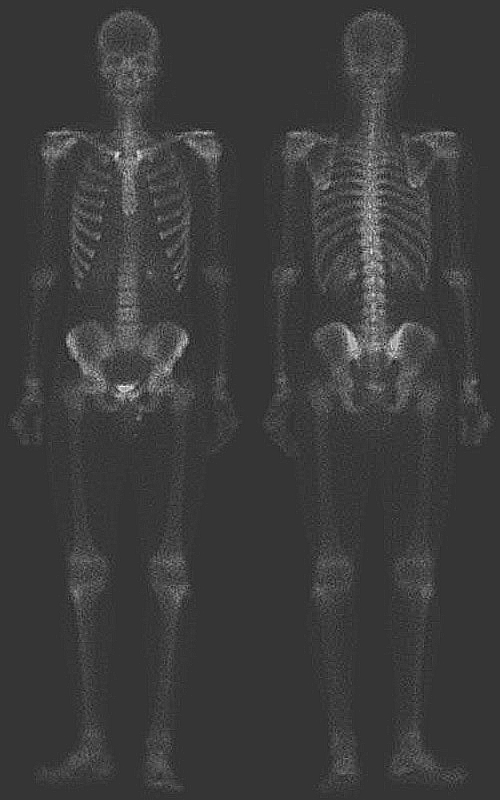
\includegraphics[width=0.4\linewidth]{./images/2/laplacian_A1.jpg}
        \caption{Laplacian (A=1)}\label{diagram:laplacian_1}
    \end{figure}

    \begin{figure}[!htb]\centering
        \begin{minipage}{0.40\textwidth}
            \frame{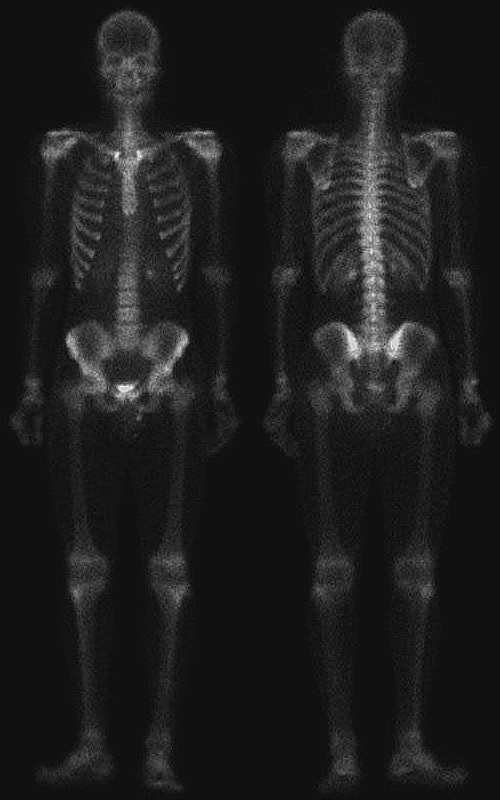
\includegraphics[width=\linewidth]{./images/2/laplacian_A1_sharpened.jpg}}
            \caption{Sharpened image}\label{diagram:laplacian_1_sharpened}
        \end{minipage}
        \begin{minipage}{0.40\textwidth}
        \frame{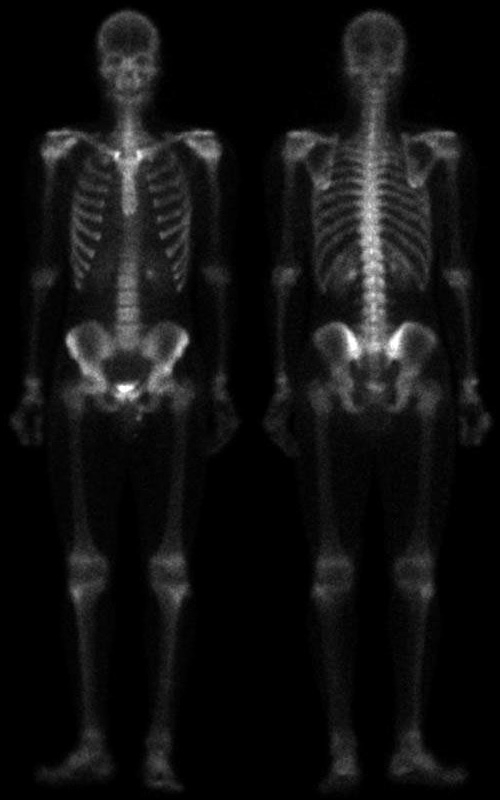
\includegraphics[width=\linewidth]{./images/2/skeleton.jpg}}
        \caption{Original image}
        \end{minipage}
    \end{figure}


    \subsection{3x3 Laplacian (A = 1.7)}

    Original image's laplacian:~\ref{diagram:laplacian_1_7} |
    Original image's sharpened laplacian:~\ref{diagram:laplacian_1_7_sharpened}

    \begin{figure}[!htb]\centering
        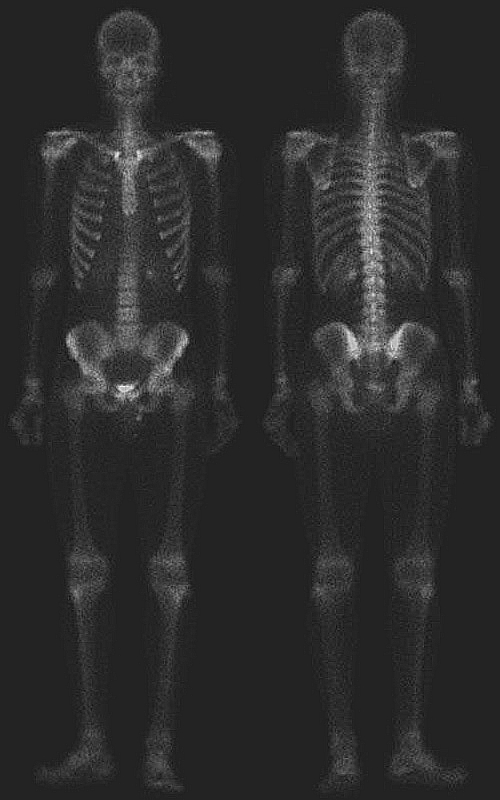
\includegraphics[width=0.4\linewidth]{./images/2/laplacian_A1-7.jpg}
        \caption{Laplacian (A=1.7)}\label{diagram:laplacian_1_7}
    \end{figure}

    \begin{figure}[!htb]\centering
        \begin{minipage}{0.40\textwidth}
            \frame{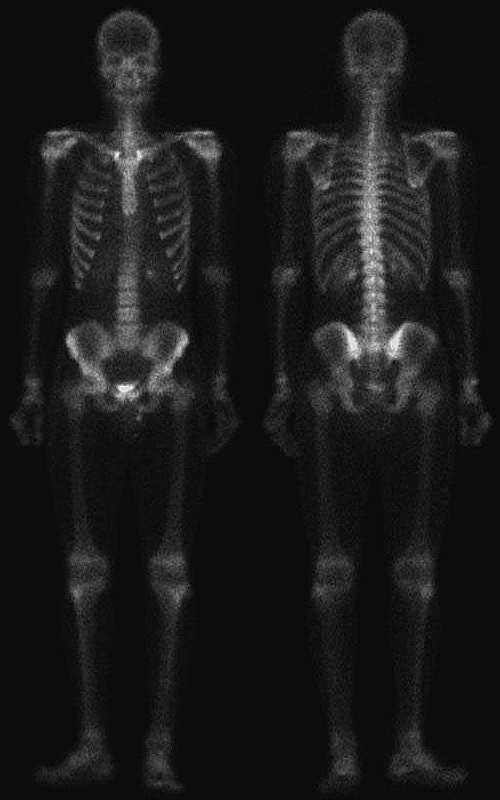
\includegraphics[width=\linewidth]{./images/2/laplacian_A1-7_sharpened.jpg}}
            \caption{Sharpened image}\label{diagram:laplacian_1_7_sharpened}
        \end{minipage}
        \begin{minipage}{0.40\textwidth}
        \frame{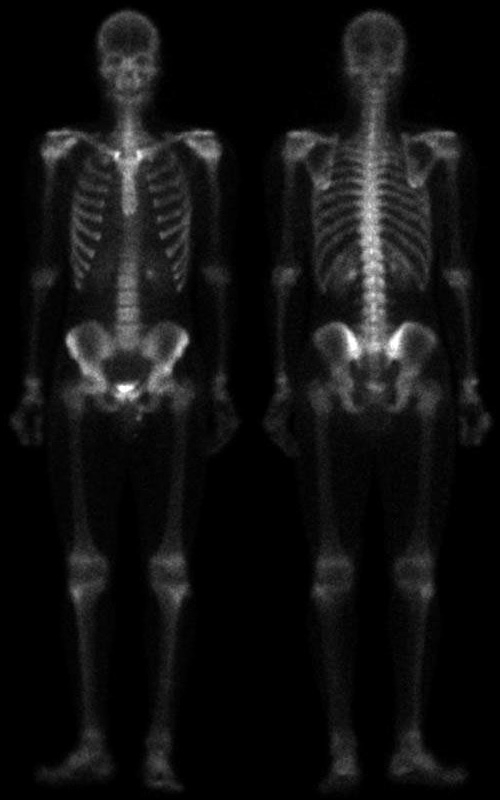
\includegraphics[width=\linewidth]{./images/2/skeleton.jpg}}
        \caption{Original image}
        \end{minipage}
    \end{figure}



    %\chapter{Filtering in frequency domain}

\section{Problem statement}

Implement the ideal, Butterworth and Gaussian lowpass and highpass filters
and test them under different parameters using \textit{characters\_test\_pattern.tif}.

\section{Python implementation}

Usage:~\textbf{python problem3.py [-h] [--ideal] [--butterworth] [--gaussian] \\
(--low | --high) [--npp] [-d D] [-n N] image\_path} \\

Use \textbf{python problem3.py -h} to see the help.

\section{Results}

    \subsection{Original image}

    \begin{figure}[!htb]\centering
        
\includegraphics[width=0.5\linewidth]{./images/3/characters.jpg}
        \caption{Original \textit{characters\_test\_pattern.tif}}
        \label{diagram:characters}
    \end{figure}


    \pagebreak
    \subsection{Ideal filter}

        \subsubsection{Low pass}

        \small{\textbf{python problem3.py --ideal -d 5 --low characters\_test\_pattern.tif}}

        \begin{figure}[!htb]\centering
            \begin{minipage}{0.45\textwidth}
                \frame{
\includegraphics[width=\linewidth]{./images/3/characters.jpg}}
                \caption{Original image}
            \end{minipage}
            \begin{minipage}{0.45\textwidth}
                \frame{
\includegraphics[width=\linewidth]{./images/3/ideal_low_5.jpg}}
                \caption{Ideal low 5}\label{diagram:ideal_low_5}
            \end{minipage}
        \end{figure}

        \begin{figure}[!htb]\centering
            \begin{minipage}{0.45\textwidth}
                \frame{
\includegraphics[width=\linewidth]{./images/3/ideal_low_15.jpg}}
                \caption{Ideal low 15}\label{diagram:ideal_low_15}
            \end{minipage}
            \begin{minipage}{0.45\textwidth}
            \frame{
\includegraphics[width=\linewidth]{./images/3/ideal_low_30.jpg}}
            \caption{Ideal low 30}\label{diagram:ideal_low_30}
            \end{minipage}
        \end{figure}

        \pagebreak
        \subsubsection{High pass}

        \small{\textbf{python problem3.py --ideal -d 5 --high characters\_test\_pattern.tif}}

        \begin{figure}[!htb]\centering
            \begin{minipage}{0.45\textwidth}
                \frame{
\includegraphics[width=\linewidth]{./images/3/characters.jpg}}
                \caption{\small{Original image}}
            \end{minipage}
            \begin{minipage}{0.45\textwidth}
                \frame{
\includegraphics[width=\linewidth]{./images/3/ideal_high_5.jpg}}
                \caption{\small{Ideal high 5}}\label{diagram:ideal_high_5}
            \end{minipage}
        \end{figure}

        \begin{figure}[!htb]\centering
            \begin{minipage}{0.45\textwidth}
                \frame{
\includegraphics[width=\linewidth]{./images/3/ideal_high_15.jpg}}
                \caption{\small{Ideal high 15}}\label{diagram:ideal_high_15}
            \end{minipage}
            \begin{minipage}{0.45\textwidth}
            \frame{
\includegraphics[width=\linewidth]{./images/3/ideal_high_30.jpg}}
            \caption{\small{Ideal high 30}}\label{diagram:ideal_high_30}
            \end{minipage}
        \end{figure}


    \pagebreak
    \subsection{Butterworth order 2 filter}

        \subsubsection{Low pass}

        \small{\textbf{python problem3.py --butterworth -d 5 -n 2 --low characters\_test\_pattern.tif}}

        \begin{figure}[!htb]\centering
            \begin{minipage}{0.45\textwidth}
                \frame{
\includegraphics[width=\linewidth]{./images/3/characters.jpg}}
                \caption{\small{Original image}}
            \end{minipage}
            \begin{minipage}{0.45\textwidth}
                \frame{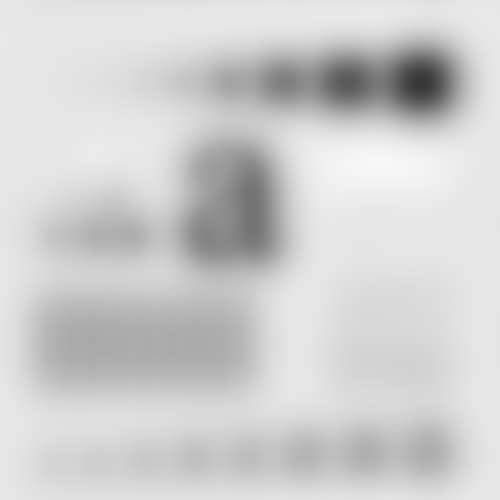
\includegraphics[width=\linewidth]{./images/3/butterworth_low_5_n2.jpg}}
                \caption{\small{Butterworth low 5}}\label{diagram:butterworth_low_5}
            \end{minipage}
        \end{figure}

        \begin{figure}[!htb]\centering
            \begin{minipage}{0.45\textwidth}
                \frame{
\includegraphics[width=\linewidth]{./images/3/butterworth_low_15_n2.jpg}}
                \caption{\small{Butterworth low 15}}\label{diagram:butterworth_low_15}
            \end{minipage}
            \begin{minipage}{0.45\textwidth}
            \frame{
\includegraphics[width=\linewidth]{./images/3/butterworth_low_30_n2.jpg}}
            \caption{\small{Butterworth low 30}}\label{diagram:butterworth_low_30}
            \end{minipage}
        \end{figure}

        \pagebreak
        \subsubsection{High pass}

        \small{\textbf{python problem3.py --butterworth -d 5 -n 2 --high characters\_test\_pattern.tif}}

        \begin{figure}[!htb]\centering
            \begin{minipage}{0.45\textwidth}
                \frame{
\includegraphics[width=\linewidth]{./images/3/characters.jpg}}
                \caption{\small{Original image}}
            \end{minipage}
            \begin{minipage}{0.45\textwidth}
                \frame{
\includegraphics[width=\linewidth]{./images/3/butterworth_high_5_n2.jpg}}
                \caption{\small{Butterworth high 5}}\label{diagram:butterworth_high_5}
            \end{minipage}
        \end{figure}

        \begin{figure}[!htb]\centering
            \begin{minipage}{0.45\textwidth}
                \frame{
\includegraphics[width=\linewidth]{./images/3/butterworth_high_15_n2.jpg}}
                \caption{\small{Butterworth high 15}}\label{diagram:butterworth_high_15}
            \end{minipage}
            \begin{minipage}{0.45\textwidth}
            \frame{
\includegraphics[width=\linewidth]{./images/3/butterworth_high_30_n2.jpg}}
            \caption{\small{Butterworth high 30}}\label{diagram:butterworth_high_30}
            \end{minipage}
        \end{figure}

    \pagebreak
    \subsection{Butterworth order 5 filter}

        \subsubsection{Low pass}

        \small{\textbf{python problem3.py --butterworth -d 5 -n 5 --low characters\_test\_pattern.tif}}

        \begin{figure}[!htb]\centering
            \begin{minipage}{0.45\textwidth}
                \frame{
\includegraphics[width=\linewidth]{./images/3/characters.jpg}}
                \caption{\small{Original image}}
            \end{minipage}
            \begin{minipage}{0.45\textwidth}
                \frame{
\includegraphics[width=\linewidth]{./images/3/butterworth_low_5_n5.jpg}}
                \caption{\small{Butterworth low 5}}\label{diagram:butterworth_low_5}
            \end{minipage}
        \end{figure}

        \begin{figure}[!htb]\centering
            \begin{minipage}{0.45\textwidth}
                \frame{
\includegraphics[width=\linewidth]{./images/3/butterworth_low_15_n5.jpg}}
                \caption{\small{Butterworth low 15}}\label{diagram:butterworth_low_15}
            \end{minipage}
            \begin{minipage}{0.45\textwidth}
            \frame{
\includegraphics[width=\linewidth]{./images/3/butterworth_low_30_n5.jpg}}
            \caption{\small{Butterworth low 30}}\label{diagram:butterworth_low_30}
            \end{minipage}
        \end{figure}

        \pagebreak
        \subsubsection{High pass}

        \small{\textbf{python problem3.py --butterworth -d 5 -n 5 --high characters\_test\_pattern.tif}}

        \begin{figure}[!htb]\centering
            \begin{minipage}{0.45\textwidth}
                \frame{
\includegraphics[width=\linewidth]{./images/3/characters.jpg}}
                \caption{\small{Original image}}
            \end{minipage}
            \begin{minipage}{0.45\textwidth}
                \frame{
\includegraphics[width=\linewidth]{./images/3/butterworth_high_5_n5.jpg}}
                \caption{\small{Butterworth high 5}}\label{diagram:butterworth_high_5}
            \end{minipage}
        \end{figure}

        \begin{figure}[!htb]\centering
            \begin{minipage}{0.45\textwidth}
                \frame{
\includegraphics[width=\linewidth]{./images/3/butterworth_high_15_n5.jpg}}
                \caption{\small{Butterworth high 15}}\label{diagram:butterworth_high_15}
            \end{minipage}
            \begin{minipage}{0.45\textwidth}
            \frame{
\includegraphics[width=\linewidth]{./images/3/butterworth_high_30_n5.jpg}}
            \caption{\small{Butterworth high 30}}\label{diagram:butterworth_high_30}
            \end{minipage}
        \end{figure}


    \pagebreak
    \subsection{Gaussian filter}

        \subsubsection{Low pass}

        \small{\textbf{python problem3.py --gaussian -d 5 --low characters\_test\_pattern.tif}}

        \begin{figure}[!htb]\centering
            \begin{minipage}{0.45\textwidth}
                \frame{
\includegraphics[width=\linewidth]{./images/3/characters.jpg}}
                \caption{Original image}
            \end{minipage}
            \begin{minipage}{0.45\textwidth}
                \frame{
\includegraphics[width=\linewidth]{./images/3/gaussian_low_5.jpg}}
                \caption{Gaussian low 5}\label{diagram:gaussian_low_5}
            \end{minipage}
        \end{figure}

        \begin{figure}[!htb]\centering
            \begin{minipage}{0.45\textwidth}
                \frame{
\includegraphics[width=\linewidth]{./images/3/gaussian_low_15.jpg}}
                \caption{Gaussian low 15}\label{diagram:gaussian_low_15}
            \end{minipage}
            \begin{minipage}{0.45\textwidth}
            \frame{
\includegraphics[width=\linewidth]{./images/3/gaussian_low_30.jpg}}
            \caption{Gaussian low 30}\label{diagram:gaussian_low_30}
            \end{minipage}
        \end{figure}

        \pagebreak
        \subsubsection{High pass}

        \small{\textbf{python problem3.py --gaussian -d 5 --high characters\_test\_pattern.tif}}

        \begin{figure}[!htb]\centering
            \begin{minipage}{0.45\textwidth}
                \frame{
\includegraphics[width=\linewidth]{./images/3/characters.jpg}}
                \caption{\small{Original image}}
            \end{minipage}
            \begin{minipage}{0.45\textwidth}
                \frame{\includegraphics[width=\linewidth]{./images/3/gaussian_high_5.jpg}}
                \caption{\small{Gaussian high 5}}\label{diagram:gaussian_high_5}
            \end{minipage}
        \end{figure}

        \begin{figure}[!htb]\centering
            \begin{minipage}{0.45\textwidth}
                \frame{\includegraphics[width=\linewidth]{./images/3/gaussian_high_15.jpg}}
                \caption{\small{Gaussian high 15}}\label{diagram:gaussian_high_15}
            \end{minipage}
            \begin{minipage}{0.45\textwidth}
            \frame{\includegraphics[width=\linewidth]{./images/3/gaussian_high_30.jpg}}
            \caption{\small{Gaussian high 30}}\label{diagram:gaussian_high_30}
            \end{minipage}
        \end{figure}

    %\chapter{Noise generation and noise reduction}

\section{Problem statement}

In this problem, you are required to write a program to generate different types
of random noises started from the Uniform noise and Gaussian noise. \\
And then add some of these noises to the circuit image and investigate the different
mean filters and order statistics as the textbook did at pages 344-352.

\section{Python implementation}

Usage:~\textbf{problem4.py [-h] (--uniform | --gaussian) [--histogram] \\}
\textbf{[--arithmetic] [--geometric] [--harmonic] [--contraharmonic] [-q Q]} \\
\textbf{[--median] [--max] [--min] [--midpoint] [--alpha] [-d D]} \\
\textbf{image\_path} \\\\
Use \textbf{python problem4.py -h} to see the help.

\pagebreak
\section{Gaussian noise}

\subsection{Noise generation and histogram}

\textbf{python problem4.py --gaussian circuit.tif}

\begin{figure}[!htb]\centering
    \includegraphics[width=0.6\linewidth]{./images/4/original.jpg}
    \caption{\small{Original image}}
\end{figure}

\begin{figure}[!htb]\centering
    \includegraphics[width=0.6\linewidth]{./images/4/gaussian_noise.jpg}
    \caption{\small{Image + Gaussian noise ($\mu = 0, \sigma = 20$)}}\label{diagram:gaussian_noise}
\end{figure}


\pagebreak
\textbf{python problem4.py --gaussian --histogram circuit.tif}

\begin{figure}[!htb]\centering
    \includegraphics[width=0.7\linewidth]{./images/4/histogram_original.jpg}
    \caption{\small{Histogram of original image}}\label{diagram:histogram_original}
\end{figure}

\begin{figure}[!htb]\centering
    \includegraphics[width=0.7\linewidth]{./images/4/histogram_gaussian.jpg}
    \caption{\small{Histogram of image with Gaussian noise}}\label{diagram:histogram_gaussian}
\end{figure}


\pagebreak
\subsection{Noise reduction}

\subsubsection{Mean filters}

\begin{minipage}{\textwidth}
\textbf{python problem4.py --gaussian --arithmetic circuit.tif} \\
\textbf{python problem4.py --gaussian --geometric circuit.tif} \\
\end{minipage}

\begin{figure}[!htb]\centering
    \begin{minipage}{0.45\textwidth}
        \frame{\includegraphics[width=\linewidth]{./images/4/original.jpg}}
        \caption{\small{Original image}}
    \end{minipage}
    \begin{minipage}{0.45\textwidth}
        \frame{\includegraphics[width=\linewidth]{./images/4/gaussian_noise.jpg}}
        \caption{\small{Image + Gaussian}}
    \end{minipage}
\end{figure}

\begin{figure}[!htb]\centering
    \begin{minipage}{0.45\textwidth}
        \frame{\includegraphics[width=\linewidth]{./images/4/gaussian_arithmetic.jpg}}
        \caption{\small{Arithmetic filter}}\label{diagram:gaussian_arithmetic}
    \end{minipage}
    \begin{minipage}{0.45\textwidth}
    \frame{\includegraphics[width=\linewidth]{./images/4/gaussian_geometric.jpg}}
    \caption{\small{Geometric filter}}\label{diagram:gaussian_geometric}
    \end{minipage}
\end{figure}

\pagebreak
\begin{minipage}{\textwidth}
\textbf{python problem4.py --gaussian --harmonic circuit.tif} \\
\end{minipage}

\begin{figure}[!htb]\centering
    \begin{minipage}{0.45\textwidth}
        \frame{\includegraphics[width=\linewidth]{./images/4/original.jpg}}
        \caption{\small{Original image}}
    \end{minipage}
    \begin{minipage}{0.45\textwidth}
        \frame{\includegraphics[width=\linewidth]{./images/4/gaussian_noise.jpg}}
        \caption{\small{Image + Gaussian}}
    \end{minipage}
\end{figure}

\begin{figure}[!htb]\centering
    \begin{minipage}{0.45\textwidth}
        \frame{\includegraphics[width=\linewidth]{./images/4/gaussian_harmonic.jpg}}
        \caption{\small{Harmonic filter}}\label{diagram:gaussian_harmonic}
    \end{minipage}
\end{figure}

\pagebreak
\begin{minipage}{\textwidth}
\textbf{python problem4.py --gaussian --contraharmonic -q 1.5 circuit.tif} \\
\textbf{python problem4.py --gaussian --contraharmonic -q -1.5 circuit.tif} \\
\end{minipage}

\begin{figure}[!htb]\centering
    \begin{minipage}{0.45\textwidth}
        \frame{\includegraphics[width=\linewidth]{./images/4/original.jpg}}
        \caption{\small{Original image}}
    \end{minipage}
    \begin{minipage}{0.45\textwidth}
        \frame{\includegraphics[width=\linewidth]{./images/4/gaussian_noise.jpg}}
        \caption{\small{Image + Gaussian}}
    \end{minipage}
\end{figure}

\begin{figure}[!htb]\centering
    \begin{minipage}{0.45\textwidth}
        \frame{\includegraphics[width=\linewidth]{./images/4/gaussian_contraharmonic_1-5.jpg}}
        \caption{\small{Contra-harmonic filter (Q=1.5)}}\label{diagram:gaussian_contraharmonic_1_5}
    \end{minipage}
    \begin{minipage}{0.45\textwidth}
        \frame{\includegraphics[width=\linewidth]{./images/4/gaussian_contraharmonic_-1-5.jpg}}
        \caption{\small{Contra-harmonic filter (Q=-1.5)}}\label{diagram:gaussian_contraharmonic_-1_5}
    \end{minipage}
\end{figure}


\pagebreak
\subsubsection{Order-Statistic filters}

\begin{minipage}{\textwidth}
\textbf{python problem4.py --gaussian --median circuit.tif} \\
\end{minipage}

\begin{figure}[!htb]\centering
    \begin{minipage}{0.45\textwidth}
        \frame{\includegraphics[width=\linewidth]{./images/4/original.jpg}}
        \caption{\small{Original image}}
    \end{minipage}
    \begin{minipage}{0.45\textwidth}
        \frame{\includegraphics[width=\linewidth]{./images/4/gaussian_noise.jpg}}
        \caption{\small{Image + Gaussian}}
    \end{minipage}
\end{figure}

\begin{figure}[!htb]\centering
    \begin{minipage}{0.45\textwidth}
        \frame{\includegraphics[width=\linewidth]{./images/4/gaussian_median.jpg}}
        \caption{\small{Median filter}}\label{diagram:gaussian_median}
    \end{minipage}
\end{figure}

\pagebreak
\begin{minipage}{\textwidth}
\textbf{python problem4.py --gaussian --max circuit.tif} \\
\textbf{python problem4.py --gaussian --min circuit.tif} \\
\end{minipage}

\begin{figure}[!htb]\centering
    \begin{minipage}{0.45\textwidth}
        \frame{\includegraphics[width=\linewidth]{./images/4/original.jpg}}
        \caption{\small{Original image}}
    \end{minipage}
    \begin{minipage}{0.45\textwidth}
        \frame{\includegraphics[width=\linewidth]{./images/4/gaussian_noise.jpg}}
        \caption{\small{Image + Gaussian}}
    \end{minipage}
\end{figure}

\begin{figure}[!htb]\centering
    \begin{minipage}{0.45\textwidth}
        \frame{\includegraphics[width=\linewidth]{./images/4/gaussian_max.jpg}}
        \caption{\small{Max filter}}\label{diagram:gaussian_max}
    \end{minipage}
    \begin{minipage}{0.45\textwidth}
        \frame{\includegraphics[width=\linewidth]{./images/4/gaussian_min.jpg}}
        \caption{\small{Min filter}}\label{diagram:gaussian_min}
    \end{minipage}
\end{figure}

\pagebreak
\begin{minipage}{\textwidth}
\textbf{python problem4.py --gaussian --midpoint circuit.tif} \\
\end{minipage}

\begin{figure}[!htb]\centering
    \begin{minipage}{0.45\textwidth}
        \frame{\includegraphics[width=\linewidth]{./images/4/original.jpg}}
        \caption{\small{Original image}}
    \end{minipage}
    \begin{minipage}{0.45\textwidth}
        \frame{\includegraphics[width=\linewidth]{./images/4/gaussian_noise.jpg}}
        \caption{\small{Image + Gaussian}}
    \end{minipage}
\end{figure}

\begin{figure}[!htb]\centering
    \begin{minipage}{0.45\textwidth}
        \frame{\includegraphics[width=\linewidth]{./images/4/gaussian_midpoint.jpg}}
        \caption{\small{Midpoint filter}}\label{diagram:gaussian_midpoint}
    \end{minipage}
\end{figure}


\pagebreak
\begin{minipage}{\textwidth}
\textbf{python problem4.py --gaussian --alpha -d 2 circuit.tif} \\
\textbf{python problem4.py --gaussian --alpha -d 4 circuit.tif} \\
\end{minipage}


\begin{figure}[!htb]\centering
    \begin{minipage}{0.45\textwidth}
        \frame{\includegraphics[width=\linewidth]{./images/4/original.jpg}}
        \caption{\small{Original image}}
    \end{minipage}
    \begin{minipage}{0.45\textwidth}
        \frame{\includegraphics[width=\linewidth]{./images/4/gaussian_noise.jpg}}
        \caption{\small{Image + Gaussian}}
    \end{minipage}
\end{figure}

\begin{figure}[!htb]\centering
    \begin{minipage}{0.45\textwidth}
        \frame{\includegraphics[width=\linewidth]{./images/4/gaussian_alpha_2.jpg}}
        \caption{\small{Alpha-trimmed filter \\(d = 2)}}\label{diagram:gaussian_alpha_2}
    \end{minipage}
    \begin{minipage}{0.45\textwidth}
        \frame{\includegraphics[width=\linewidth]{./images/4/gaussian_alpha_4.jpg}}
        \caption{\small{Alpha-trimmed filter \\(d = 4)}}\label{diagram:gaussian_alpha_4}
    \end{minipage}
\end{figure}


\pagebreak
\section{Uniform noise}

\subsection{Noise generation and histogram}

\textbf{python problem4.py --uniform circuit.tif}

\begin{figure}[!htb]\centering
    \includegraphics[width=0.6\linewidth]{./images/4/original.jpg}
    \caption{\small{Original image}}
\end{figure}

\begin{figure}[!htb]\centering
    \includegraphics[width=0.6\linewidth]{./images/4/uniform_noise.jpg}
    \caption{\small{Image + Uniform noise (min = 0, max = 128)}}\label{diagram:uniform_noise}
\end{figure}


\pagebreak
\textbf{python problem4.py --uniform --histogram circuit.tif}

\begin{figure}[!htb]\centering
    \includegraphics[width=0.7\linewidth]{./images/4/histogram_original.jpg}
    \caption{\small{Histogram of original image}}\label{diagram:histogram_original}
\end{figure}

\begin{figure}[!htb]\centering
    \includegraphics[width=0.7\linewidth]{./images/4/histogram_uniform.jpg}
    \caption{\small{Histogram of image with Uniform noise}}\label{diagram:histogram_uniform}
\end{figure}


\pagebreak
\subsection{Noise reduction}

\subsubsection{Mean filters}

\begin{minipage}{\textwidth}
\textbf{python problem4.py --uniform --arithmetic circuit.tif} \\
\textbf{python problem4.py --uniform --geometric circuit.tif} \\
\end{minipage}

\begin{figure}[!htb]\centering
    \begin{minipage}{0.45\textwidth}
        \frame{\includegraphics[width=\linewidth]{./images/4/original.jpg}}
        \caption{\small{Original image}}
    \end{minipage}
    \begin{minipage}{0.45\textwidth}
        \frame{\includegraphics[width=\linewidth]{./images/4/uniform_noise.jpg}}
        \caption{\small{Image + Uniform}}
    \end{minipage}
\end{figure}

\begin{figure}[!htb]\centering
    \begin{minipage}{0.45\textwidth}
        \frame{\includegraphics[width=\linewidth]{./images/4/uniform_arithmetic.jpg}}
        \caption{\small{Arithmetic filter}}\label{diagram:uniform_arithmetic}
    \end{minipage}
    \begin{minipage}{0.45\textwidth}
    \frame{\includegraphics[width=\linewidth]{./images/4/uniform_geometric.jpg}}
    \caption{\small{Geometric filter}}\label{diagram:uniform_geometric}
    \end{minipage}
\end{figure}

\pagebreak
\begin{minipage}{\textwidth}
\textbf{python problem4.py --uniform --harmonic circuit.tif} \\
\end{minipage}

\begin{figure}[!htb]\centering
    \begin{minipage}{0.45\textwidth}
        \frame{\includegraphics[width=\linewidth]{./images/4/original.jpg}}
        \caption{\small{Original image}}
    \end{minipage}
    \begin{minipage}{0.45\textwidth}
        \frame{\includegraphics[width=\linewidth]{./images/4/uniform_noise.jpg}}
        \caption{\small{Image + Uniform}}
    \end{minipage}
\end{figure}

\begin{figure}[!htb]\centering
    \begin{minipage}{0.45\textwidth}
        \frame{\includegraphics[width=\linewidth]{./images/4/uniform_harmonic.jpg}}
        \caption{\small{Harmonic filter}}\label{diagram:uniform_harmonic}
    \end{minipage}
\end{figure}

\pagebreak
\begin{minipage}{\textwidth}
\textbf{python problem4.py --uniform --contraharmonic -q 1.5 circuit.tif} \\
\textbf{python problem4.py --uniform --contraharmonic -q -1.5 circuit.tif} \\
\end{minipage}

\begin{figure}[!htb]\centering
    \begin{minipage}{0.45\textwidth}
        \frame{\includegraphics[width=\linewidth]{./images/4/original.jpg}}
        \caption{\small{Original image}}
    \end{minipage}
    \begin{minipage}{0.45\textwidth}
        \frame{\includegraphics[width=\linewidth]{./images/4/uniform_noise.jpg}}
        \caption{\small{Image + Uniform}}
    \end{minipage}
\end{figure}

\begin{figure}[!htb]\centering
    \begin{minipage}{0.45\textwidth}
        \frame{\includegraphics[width=\linewidth]{./images/4/uniform_contraharmonic_1-5.jpg}}
        \caption{\small{Contra-harmonic filter (Q=1.5)}}\label{diagram:uniform_contraharmonic_1_5}
    \end{minipage}
    \begin{minipage}{0.45\textwidth}
        \frame{\includegraphics[width=\linewidth]{./images/4/uniform_contraharmonic_-1-5.jpg}}
        \caption{\small{Contra-harmonic filter (Q=-1.5)}}\label{diagram:uniform_contraharmonic_-1_5}
    \end{minipage}
\end{figure}


\pagebreak
\subsubsection{Order-Statistic filters}

\begin{minipage}{\textwidth}
\textbf{python problem4.py --uniform --median circuit.tif} \\
\end{minipage}

\begin{figure}[!htb]\centering
    \begin{minipage}{0.45\textwidth}
        \frame{\includegraphics[width=\linewidth]{./images/4/original.jpg}}
        \caption{\small{Original image}}
    \end{minipage}
    \begin{minipage}{0.45\textwidth}
        \frame{\includegraphics[width=\linewidth]{./images/4/uniform_noise.jpg}}
        \caption{\small{Image + Uniform}}
    \end{minipage}
\end{figure}

\begin{figure}[!htb]\centering
    \begin{minipage}{0.45\textwidth}
        \frame{\includegraphics[width=\linewidth]{./images/4/uniform_median.jpg}}
        \caption{\small{Median filter}}\label{diagram:uniform_median}
    \end{minipage}
\end{figure}

\pagebreak
\begin{minipage}{\textwidth}
\textbf{python problem4.py --uniform --max circuit.tif} \\
\textbf{python problem4.py --uniform --min circuit.tif} \\
\end{minipage}

\begin{figure}[!htb]\centering
    \begin{minipage}{0.45\textwidth}
        \frame{\includegraphics[width=\linewidth]{./images/4/original.jpg}}
        \caption{\small{Original image}}
    \end{minipage}
    \begin{minipage}{0.45\textwidth}
        \frame{\includegraphics[width=\linewidth]{./images/4/uniform_noise.jpg}}
        \caption{\small{Image + Uniform}}
    \end{minipage}
\end{figure}

\begin{figure}[!htb]\centering
    \begin{minipage}{0.45\textwidth}
        \frame{\includegraphics[width=\linewidth]{./images/4/uniform_max.jpg}}
        \caption{\small{Max filter}}\label{diagram:uniform_max}
    \end{minipage}
    \begin{minipage}{0.45\textwidth}
        \frame{\includegraphics[width=\linewidth]{./images/4/uniform_min.jpg}}
        \caption{\small{Min filter}}\label{diagram:uniform_min}
    \end{minipage}
\end{figure}

\pagebreak
\begin{minipage}{\textwidth}
\textbf{python problem4.py --uniform --midpoint circuit.tif} \\
\end{minipage}

\begin{figure}[!htb]\centering
    \begin{minipage}{0.45\textwidth}
        \frame{\includegraphics[width=\linewidth]{./images/4/original.jpg}}
        \caption{\small{Original image}}
    \end{minipage}
    \begin{minipage}{0.45\textwidth}
        \frame{\includegraphics[width=\linewidth]{./images/4/uniform_noise.jpg}}
        \caption{\small{Image + Uniform}}
    \end{minipage}
\end{figure}

\begin{figure}[!htb]\centering
    \begin{minipage}{0.45\textwidth}
        \frame{\includegraphics[width=\linewidth]{./images/4/uniform_midpoint.jpg}}
        \caption{\small{Midpoint filter}}\label{diagram:uniform_midpoint}
    \end{minipage}
\end{figure}


\pagebreak
\begin{minipage}{\textwidth}
\textbf{python problem4.py --uniform --alpha -d 2 circuit.tif} \\
\textbf{python problem4.py --uniform --alpha -d 4 circuit.tif} \\
\end{minipage}


\begin{figure}[!htb]\centering
    \begin{minipage}{0.45\textwidth}
        \frame{\includegraphics[width=\linewidth]{./images/4/original.jpg}}
        \caption{\small{Original image}}
    \end{minipage}
    \begin{minipage}{0.45\textwidth}
        \frame{\includegraphics[width=\linewidth]{./images/4/uniform_noise.jpg}}
        \caption{\small{Image + Uniform}}
    \end{minipage}
\end{figure}

\begin{figure}[!htb]\centering
    \begin{minipage}{0.45\textwidth}
        \frame{\includegraphics[width=\linewidth]{./images/4/uniform_alpha_2.jpg}}
        \caption{\small{Alpha-trimmed filter \\(d = 2)}}\label{diagram:uniform_alpha_2}
    \end{minipage}
    \begin{minipage}{0.45\textwidth}
        \frame{\includegraphics[width=\linewidth]{./images/4/uniform_alpha_4.jpg}}
        \caption{\small{Alpha-trimmed filter \\(d = 4)}}\label{diagram:uniform_alpha_4}
    \end{minipage}
\end{figure}

    %\chapter{Image restoration}

\section{Problem statement}

Suppose a blurring degradation function as
\begin{equation}
    H(u, v) = T \times sinc(ua + vb) \times e^{-j\pi(ua + vb)}
\end{equation}
\bigskip
\begin{enumerate}[(a)]
    \item Implement a blurring filter using the equation above.
    \item Blur the test image book\_cover.jpg using parameters $a = b = 0.1$ and $T = 1$.
    \item Add Gaussian noise of $0$ mean and variance of $650$ to the blurred image.
    \item Restore the blurred image and the blurred noisy image using the inverse filter,
          Wiener deconvolution filter and the parametric Wiener filter, respectively.
      \item Add Gaussian noise of $0$ and different variances to the blurred image and repeat (d),
          investigate the performance of the Wiener deconvolution filter.
\end{enumerate}

\section{Python implementation}

Usage:~\textbf{problem5.py [-h] [--blurred BLURRED] [--noise] [-s S] [--inv]} \\
\textbf{[--wiener] [-a A] [-b B] [-T T] [-K K]}
\textbf{image\_path} \\\\
Use \textbf{python problem5.py -h} to see the help.

\pagebreak
\section{Blurring and noising}

\textbf{python problem5.py book\_cover.jpg}

\begin{figure}[!htb]\centering
    \includegraphics[width=0.6\linewidth]{./images/5/original.jpg}
    \caption{\small{Original image}}
\end{figure}

\begin{figure}[!htb]\centering
    \includegraphics[width=0.6\linewidth]{./images/5/blurred.jpg}
    \caption{\small{Blurred image ($a = b = 0.1; T = 1$)}}\label{diagram:blurred}
\end{figure}


\pagebreak
\textbf{python problem5.py book\_cover.jpg --noise -s 650}

\begin{figure}[!htb]\centering
    \includegraphics[width=0.6\linewidth]{./images/5/blurred_noise.jpg}
    \caption{\small{Blur + Gaussian noise ($\mu = 0, \sigma^2 = 650$)}}\label{diagram:blurred_noise}
\end{figure}


\pagebreak
\section{Restoration}

\subsection{Inverse filter}

\begin{minipage}{\textwidth}
\textbf{python problem5.py --inv book\_cover.jpg} \\
\textbf{python problem5.py --noise -s 650 --inv book\_cover.jpg}
\end{minipage}

\begin{figure}[!htb]\centering
    \begin{minipage}{0.45\textwidth}
        \frame{\includegraphics[width=\linewidth]{./images/5/blurred.jpg}}
        \caption{\small{Blurred image}}
    \end{minipage}
    \begin{minipage}{0.45\textwidth}
        \frame{\includegraphics[width=\linewidth]{./images/5/inv_blurred.jpg}}
        \caption{\small{Inverse blurred image}}\label{diagram:inv_blurred}
    \end{minipage}
\end{figure}

\begin{figure}[!htb]\centering
    \begin{minipage}{0.45\textwidth}
        \frame{\includegraphics[width=\linewidth]{./images/5/blurred_noise.jpg}}
        \caption{\small{Blur + noise}}
    \end{minipage}
    \begin{minipage}{0.45\textwidth}
    \frame{\includegraphics[width=\linewidth]{./images/5/inv_blurred_noise.jpg}}
    \caption{\small{Inverse 'blur + noise'}}\label{diagram:inv_blurred_noise}
    \end{minipage}
\end{figure}
\bigskip
The inverse filter is really affected by the noise because it ignores it (does not inverse it).

\pagebreak
\subsection{Wiener filter}
\begin{minipage}{\textwidth}
\textbf{python problem5.py --wiener book\_cover.jpg} \\
\textbf{python problem5.py --noise -s 650 --wiener book\_cover.jpg}
\end{minipage}

\begin{figure}[!htb]\centering
    \begin{minipage}{0.45\textwidth}
        \frame{\includegraphics[width=\linewidth]{./images/5/blurred.jpg}}
        \caption{\small{Blurred image}}
    \end{minipage}
    \begin{minipage}{0.45\textwidth}
        \frame{\includegraphics[width=\linewidth]{./images/5/wiener_blurred.jpg}}
        \caption{\small{Wiener blurred image}}\label{diagram:wiener_blurred}
    \end{minipage}
\end{figure}

\begin{figure}[!htb]\centering
    \begin{minipage}{0.45\textwidth}
        \frame{\includegraphics[width=\linewidth]{./images/5/blurred_noise.jpg}}
        \caption{\small{Blur + noise}}
    \end{minipage}
    \begin{minipage}{0.45\textwidth}
    \frame{\includegraphics[width=\linewidth]{./images/5/wiener_blurred_noise.jpg}}
    \caption{\small{Wiener 'blur + noise'}}\label{diagram:wiener_blurred_noise}
    \end{minipage}
\end{figure}
\bigskip
The Wiener filter on the blurred image without noise is equivalent to the inverse filter (power spectrum of noise equals to 0). \\
The Wiener filter is more efficient to remove the noise as it takes it into consideration
during the restoration process.

\pagebreak
\subsection{Parametric Wiener filter}
TODO

\pagebreak
\subsection{Experimentations}

\subsubsection{Gaussian noise ($\mu = 0, \sigma^2 = 300$)}

\begin{figure}[!htb]\centering
    \begin{minipage}{0.45\textwidth}
        \frame{\includegraphics[width=\linewidth]{./images/5/original.jpg}}
        \caption{\small{Original image}}
    \end{minipage}
    \begin{minipage}{0.45\textwidth}
        \frame{\includegraphics[width=\linewidth]{./images/5/blurred_noise_300.jpg}}
        \caption{\small{Blur + noise}}
    \end{minipage}
\end{figure}

\begin{figure}[!htb]\centering
    \begin{minipage}{0.45\textwidth}
        \frame{\includegraphics[width=\linewidth]{./images/5/inv_blurred_noise_300.jpg}}
        \caption{\small{Inverse 'blur + noise'}}
    \end{minipage}
    \begin{minipage}{0.45\textwidth}
    \frame{\includegraphics[width=\linewidth]{./images/5/wiener_blurred_noise_300.jpg}}
    \caption{\small{Wiener 'blur + noise'}}
    \end{minipage}
\end{figure}

\pagebreak
\subsubsection{Gaussian noise ($\mu = 0, \sigma^2 = 100$)}

\begin{figure}[!htb]\centering
    \begin{minipage}{0.45\textwidth}
        \frame{\includegraphics[width=\linewidth]{./images/5/original.jpg}}
        \caption{\small{Original image}}
    \end{minipage}
    \begin{minipage}{0.45\textwidth}
        \frame{\includegraphics[width=\linewidth]{./images/5/blurred_noise_100.jpg}}
        \caption{\small{Blur + noise}}
    \end{minipage}
\end{figure}

\begin{figure}[!htb]\centering
    \begin{minipage}{0.45\textwidth}
        \frame{\includegraphics[width=\linewidth]{./images/5/inv_blurred_noise_100.jpg}}
        \caption{\small{Inverse 'blur + noise'}}
    \end{minipage}
    \begin{minipage}{0.45\textwidth}
    \frame{\includegraphics[width=\linewidth]{./images/5/wiener_blurred_noise_100.jpg}}
    \caption{\small{Wiener 'blur + noise'}}
    \end{minipage}
\end{figure}

\pagebreak
\subsubsection{Gaussian noise ($\mu = 0, \sigma^2 = 30$)}

\begin{figure}[!htb]\centering
    \begin{minipage}{0.45\textwidth}
        \frame{\includegraphics[width=\linewidth]{./images/5/original.jpg}}
        \caption{\small{Original image}}
    \end{minipage}
    \begin{minipage}{0.45\textwidth}
        \frame{\includegraphics[width=\linewidth]{./images/5/blurred_noise_30.jpg}}
        \caption{\small{Blur + noise}}
    \end{minipage}
\end{figure}

\begin{figure}[!htb]\centering
    \begin{minipage}{0.45\textwidth}
        \frame{\includegraphics[width=\linewidth]{./images/5/inv_blurred_noise_30.jpg}}
        \caption{\small{Inverse 'blur + noise'}}
    \end{minipage}
    \begin{minipage}{0.45\textwidth}
    \frame{\includegraphics[width=\linewidth]{./images/5/wiener_blurred_noise_30.jpg}}
    \caption{\small{Wiener 'blur + noise'}}
    \end{minipage}
\end{figure}


\pagebreak
\subsubsection{Wiener performance}

\begin{figure}[!htb]\centering
    \begin{minipage}{0.45\textwidth}
        \frame{\includegraphics[width=\linewidth]{./images/5/wiener_blurred_noise_30.jpg}}
        \caption{\small{Wiener 'blur + noise ($\sigma^2 = 30$)'}}
    \end{minipage}
    \begin{minipage}{0.45\textwidth}
        \frame{\includegraphics[width=\linewidth]{./images/5/wiener_blurred_noise_100.jpg}}
        \caption{\small{Wiener 'blur + noise ($\sigma^2 = 100$)'}}
    \end{minipage}
\end{figure}

\begin{figure}[!htb]\centering
    \begin{minipage}{0.45\textwidth}
        \frame{\includegraphics[width=\linewidth]{./images/5/wiener_blurred_noise_300.jpg}}
        \caption{\small{Inverse 'blur + noise ($\sigma^2 = 300$)'}}
    \end{minipage}
    \begin{minipage}{0.45\textwidth}
    \frame{\includegraphics[width=\linewidth]{./images/5/wiener_blurred_noise.jpg}}
    \caption{\small{Wiener 'blur + noise ($\sigma^2 = 650$)'}}
    \end{minipage}
\end{figure}

    %\chapter{Geometric transforms}

\section{Problem statement}

Develop a geometric transform program that will rotate, translate,
and scale an image by specified amounts, using the nearest neighbor
and bilinear interpolation methods, respectively.

\section{Python implementation}

Usage:~\textbf{problem6.py [-h] -i INPUT} \\
       \textbf{(-t TRANSLATE [TRANSLATE ...] | -r ROTATE | -s SCALE)}
       \textbf{(--nearest | --bilinear) [--ntruncate] [--debug]}

Use \textbf{python problem6.py -h} to see the help.

\pagebreak

\begin{figure}[!htb]\centering
    \includegraphics[width=0.6\linewidth]{./images/6/original.png}
    \caption{\small{Original image}}
\end{figure}


\pagebreak

\section{Translation}

\textbf{python problem6.py -i ray\_trace\_bottle.tif --bilinear -t tx ty}, where (tx, ty) is the 2D translation vector.

\begin{figure}[!htb]\centering
    \begin{minipage}{0.6\textwidth}
        \frame{\includegraphics[width=\linewidth]{./images/6/translate_0_300_nn.png}}
        \caption{\small{Translation (0, 300) nearest}}
    \end{minipage}
\end{figure}

\begin{figure}[!htb]\centering
    \begin{minipage}{0.6\textwidth}
    \frame{\includegraphics[width=\linewidth]{./images/6/translate_0_300_bl.png}}
    \caption{\small{Translate (0, 300) bilinear}}
    \end{minipage}
\end{figure}

\pagebreak

\begin{figure}[!htb]\centering
    \begin{minipage}{0.6\textwidth}
        \frame{\includegraphics[width=\linewidth]{./images/6/translate_250_-100_nn.png}}
        \caption{\small{Translation (250, -100) nearest}}
    \end{minipage}
\end{figure}

\begin{figure}[!htb]\centering
    \begin{minipage}{0.6\textwidth}
    \frame{\includegraphics[width=\linewidth]{./images/6/translate_250_-100_bl.png}}
    \caption{\small{Translate (250, -100) bilinear}}
    \end{minipage}
\end{figure}

\pagebreak

\begin{figure}[!htb]\centering
    \begin{minipage}{0.6\textwidth}
        \frame{\includegraphics[width=\linewidth]{./images/6/translate_109_8_75_5_nn.png}}
        \caption{\small{Translation (109.8, 75.5) nearest}}
    \end{minipage}
\end{figure}

\begin{figure}[!htb]\centering
    \begin{minipage}{0.6\textwidth}
    \frame{\includegraphics[width=\linewidth]{./images/6/translate_109_8_75_5_bl.png}}
    \caption{\small{Translation (109.8, 75.5) bilinear}}
    \end{minipage}
\end{figure}


\pagebreak

\section{Rotation}

\textbf{python problem6.py -i ray\_trace\_bottle.tif --nearest -r theta}, where theta is the angle of rotation.

\begin{figure}[!htb]\centering
    \begin{minipage}{0.6\textwidth}
        \frame{\includegraphics[width=\linewidth]{./images/6/rotate_20_nn.png}}
        \caption{\small{Rotate 20° nearest}}
    \end{minipage}
\end{figure}

\begin{figure}[!htb]\centering
    \begin{minipage}{0.6\textwidth}
    \frame{\includegraphics[width=\linewidth]{./images/6/rotate_20_bl.png}}
    \caption{\small{Rotate 20° bilinear}}
    \end{minipage}
\end{figure}

\pagebreak

\begin{figure}[!htb]\centering
    \begin{minipage}{0.6\textwidth}
        \frame{\includegraphics[width=\linewidth]{./images/6/rotate_90_nn.png}}
        \caption{\small{Rotate 90° nearest}}
    \end{minipage}
\end{figure}

\begin{figure}[!htb]\centering
    \begin{minipage}{0.6\textwidth}
    \frame{\includegraphics[width=\linewidth]{./images/6/rotate_90_bl.png}}
    \caption{\small{Rotate 90° bilinear}}
    \end{minipage}
\end{figure}


\pagebreak

\begin{figure}[!htb]\centering
    \begin{minipage}{0.6\textwidth}
        \frame{\includegraphics[width=\linewidth]{./images/6/rotate_130_nn.png}}
        \caption{\small{Rotate 130° nearest}}
    \end{minipage}
\end{figure}

\begin{figure}[!htb]\centering
    \begin{minipage}{0.6\textwidth}
    \frame{\includegraphics[width=\linewidth]{./images/6/rotate_130_bl.png}}
    \caption{\small{Rotate 130° bilinear}}
    \end{minipage}
\end{figure}

\pagebreak

\section{Scaling}

\begin{figure}[!htb]\centering
    \begin{minipage}{0.6\textwidth}
        \frame{\includegraphics[width=\linewidth]{./images/6/scale_0_5_nn.png}}
        \caption{\small{Scaling 0.5 nearest}}
    \end{minipage}
\end{figure}

\begin{figure}[!htb]\centering
    \begin{minipage}{0.6\textwidth}
    \frame{\includegraphics[width=\linewidth]{./images/6/scale_0_5_bl.png}}
    \caption{\small{Scaling 0.5 bilinear}}
    \end{minipage}
\end{figure}

\pagebreak

\begin{figure}[!htb]\centering
    \begin{minipage}{0.6\textwidth}
        \frame{\includegraphics[width=\linewidth]{./images/6/scale_1_5_nn.png}}
        \caption{\small{Scaling 1.5 nearest}}
    \end{minipage}
\end{figure}

\begin{figure}[!htb]\centering
    \begin{minipage}{0.6\textwidth}
    \frame{\includegraphics[width=\linewidth]{./images/6/scale_1_5_bl.png}}
    \caption{\small{Scaling 1.5 bilinear}}
    \end{minipage}
\end{figure}

\pagebreak

\begin{figure}[!htb]\centering
    \begin{minipage}{0.6\textwidth}
        \frame{\includegraphics[width=\linewidth]{./images/6/scale_2_3_nn.png}}
        \caption{\small{Scaling 2.3 nearest}}
    \end{minipage}
\end{figure}

\begin{figure}[!htb]\centering
    \begin{minipage}{0.6\textwidth}
    \frame{\includegraphics[width=\linewidth]{./images/6/scale_2_3_bl.png}}
    \caption{\small{Scaling 2.3 bilinear}}
    \end{minipage}
\end{figure}

    \chapter{Transform image compression}

\section{Problem statement}

\begin{enumerate}[(a)]
    \item Investigate image compression based on DCT.
          Divide the image into 8-by-8 subimages, compute the two-dimensional discrete cosine
          transform of each subimage, compress the test image to different qualities by
          discarding some DCT coefficients based on zonal mask
          and threshold mask and using the inverse discrete cosine
          transform with fewer transform coefficients. Display the
          original image, the reconstructed images and the
          difference images.

    \item Investigate image compression based on wavelets. \\
          Consider four types of wavelets:
          \begin{enumerate}
            \item Haar (2x2)
            \item Daubechies (8-tap)
            \item Symlet (8-tap)
            \item Cohen-Daubechies-Feauveau (17-tap)
          \end{enumerate}
\end{enumerate}

\section{Python implementation}
\bigskip
Two programs: \\
\begin{itemize}
    \item DCT compression: \textbf{dct.py}
    \item Wavelet compression: \textbf{wavelet.py}
\end{itemize}

\textbf{DCT}: \\
Usage:~\textbf{dct.py [-h] [--zonal | --threshold] [-z Z] image\_path} \\
Use \textbf{python dct.py -h} to see the help.

\bigskip

TODO: Wavelet
\textbf{Wavelet}: \\
Use \textbf{python wavelet.py -h} to see the help.

\pagebreak

\begin{figure}[!htb]\centering
    \includegraphics[width=0.6\linewidth]{./images/7/original.jpg}
    \caption{\small{Original image}}
\end{figure}

\pagebreak

\section{Image compression based on DCT}

\subsection{Zonal mask}

\textbf{python dct.py --zonal -z Z lenna.tif} where $Z = 1, 4$ or $7$.
\newline
\newline
Example: Zonal 5
\begin{equation}
\begin{bmatrix}
       1 & 1 & 1 & 1 & 1 & 0 & 0 & 0 \\
       1 & 1 & 1 & 1 & 0 & 0 & 0 & 0 \\
       1 & 1 & 1 & 0 & 0 & 0 & 0 & 0 \\
       1 & 1 & 0 & 0 & 0 & 0 & 0 & 0 \\
       1 & 0 & 0 & 0 & 0 & 0 & 0 & 0 \\
       0 & 0 & 0 & 0 & 0 & 0 & 0 & 0 \\
       0 & 0 & 0 & 0 & 0 & 0 & 0 & 0 \\
       0 & 0 & 0 & 0 & 0 & 0 & 0 & 0 \\
\end{bmatrix}
\end{equation}
\bigskip
Example: Zonal 2
\begin{equation}
\begin{bmatrix}
       1 & 1 & 0 & 0 & 0 & 0 & 0 & 0 \\
       1 & 0 & 0 & 0 & 0 & 0 & 0 & 0 \\
       0 & 0 & 0 & 0 & 0 & 0 & 0 & 0 \\
       0 & 0 & 0 & 0 & 0 & 0 & 0 & 0 \\
       0 & 0 & 0 & 0 & 0 & 0 & 0 & 0 \\
       0 & 0 & 0 & 0 & 0 & 0 & 0 & 0 \\
       0 & 0 & 0 & 0 & 0 & 0 & 0 & 0 \\
       0 & 0 & 0 & 0 & 0 & 0 & 0 & 0 \\
\end{bmatrix}
\end{equation}

\begin{figure}[!htb]\centering
    \begin{minipage}{0.45\textwidth}
        \frame{\includegraphics[width=\linewidth]{./images/7/dct_zonal_7.jpg}}
        \caption{\small{Zonal 7}}
    \end{minipage}
    \begin{minipage}{0.45\textwidth}
        \frame{\includegraphics[width=\linewidth]{./images/7/dct_zonal_7_diff.jpg}}
        \caption{\small{Zonal 7 - Diff}}
    \end{minipage}
\end{figure}

\pagebreak

\begin{figure}[!htb]\centering
    \begin{minipage}{0.4\textwidth}
        \frame{\includegraphics[width=\linewidth]{./images/7/dct_zonal_4.jpg}}
        \caption{\small{Zonal 4}}
    \end{minipage}
    \begin{minipage}{0.4\textwidth}
        \frame{\includegraphics[width=\linewidth]{./images/7/dct_zonal_4_diff.jpg}}
        \caption{\small{Zonal 4 - Diff}}
    \end{minipage}
\end{figure}

\begin{figure}[!htb]\centering
    \begin{minipage}{0.4\textwidth}
        \frame{\includegraphics[width=\linewidth]{./images/7/dct_zonal_2.jpg}}
        \caption{\small{Zonal 2}}
    \end{minipage}
    \begin{minipage}{0.4\textwidth}
        \frame{\includegraphics[width=\linewidth]{./images/7/dct_zonal_2_diff.jpg}}
        \caption{\small{Zonal 2 - Diff}}
    \end{minipage}
\end{figure}


\begin{figure}[!htb]\centering
    \begin{minipage}{0.4\textwidth}
        \frame{\includegraphics[width=\linewidth]{./images/7/dct_zonal_1.jpg}}
        \caption{\small{Zonal 1}}
    \end{minipage}
    \begin{minipage}{0.4\textwidth}
        \frame{\includegraphics[width=\linewidth]{./images/7/dct_zonal_1_diff.jpg}}
        \caption{\small{Zonal 1 - Diff}}
    \end{minipage}
\end{figure}

\pagebreak



    % ------------------------------------------------------------------- FOOTER
\end{document}
